\documentclass[11pt,a4paper,onecolumn]{IEEEtran}

\usepackage[english]{babel}
\usepackage{microtype}
\usepackage{booktabs}
\usepackage{array}
\usepackage{amsmath}
\usepackage{graphicx}
\usepackage{adjustbox}
\usepackage[nocompress]{cite}
\usepackage{hyperref}
\usepackage{xcolor}

\newcommand{\articleTitle}{Evidence-Grounded Local Language Models and Behavioral Telemetry for Defensive Network Review}
\hypersetup{
  unicode=true,
  pdfencoding=auto,
  hidelinks,
  pdftitle={\articleTitle},
  pdfauthor={João Vitor Ielen and Vinicius Mota Favaro},
  pdfsubject={Evidence-grounded defensive network review},
  pdfkeywords={network telemetry, local language model, behavioral detection, CTU-13, defensive automation}
}
\def\UrlLeft{}
\def\UrlRight{}
\setlength{\emergencystretch}{2em}
\renewcommand{\thesection}{\arabic{section}}
\renewcommand{\thesubsection}{\thesection.\arabic{subsection}}
\renewcommand{\thetable}{\arabic{table}}

\begin{document}
\bstctlcite{BSTcontrol}
\title{\articleTitle}
\author{João Vitor Ielen and Vinicius Mota Favaro\\
\normalsize Centro Universitário UniOpet, Curitiba, Paraná, Brazil\\
\normalsize Academic advisor: Michel Cesar dos Santos}
\maketitle

\begin{abstract}
Security telemetry contains observable events, not proof of compromise. This study asks whether local language models can prioritize transparent behavioral findings while preserving evidence boundaries and withholding response authority. The artifact correlates authorized Nmap inventory with normalized telemetry, applies four auditable rules, assigns stable evidence identifiers, and validates schema-constrained output deterministically. Evaluation combines inert fixtures, family-separated CTU-13 sources, a synthetic implementation-transfer source, a 180-call three-model/three-prompt matrix, adversarial pairs, and component ablations. The inert benchmark reached F1 0.889. An inspected NSIS.ay holdout reached F1 0.317 and a Matthews correlation coefficient (MCC) of -0.282; a prospectively frozen DonBot holdout reached F1 0.600 and MCC 0.452. On NSIS.ay, block-on-alert would have acted on 32 normal windows and missed 37 botnet windows. A single-model comparison retained exact identifiers in 50/50 grounded calls and 0/50 reconstructed free-text calls. In the broader matrix, 145/180 calls received responses and 73 passed deterministic validation; 35 Qwen attempts failed after the local server exited. Removing the API format constraint yielded no valid JSON in 12 calls. Among 11 adversarial pairs with both responses, validator status changed in eight. These results justify model-assisted triage only when deterministic checks remain in control. They do not support autonomous attribution or containment.
\end{abstract}

\begin{IEEEkeywords}
network telemetry, local language model, behavioral detection, CTU-13, defensive automation
\end{IEEEkeywords}

\section{Introduction}

Network discovery and operating-system telemetry describe different layers of a security event. Nmap can identify reachable hosts, open ports, and uncertain service fingerprints \cite{lyon2009,nmapdocs2025}; endpoint telemetry can associate connections, DNS queries, and file creation with processes \cite{sysmonevents2026}. Neither source alone establishes that software is malicious or that a vulnerability is exploitable. Those conclusions require provenance, context, and independent validation.

Large language models (LLMs) can organize evidence and make technical output easier to review, but fluent text can also erase the distinction between an observation and a conclusion. Local inference reduces disclosure to external services, not epistemic risk. The NIST AI Risk Management Framework emphasizes governance, measurement, and continued risk management instead of treating model output as self-validating \cite{nistai1001}.

The starting point was an undergraduate project approved in 2025. That system parsed authorized Nmap XML, produced reports, optionally requested local Ollama narratives, and proposed future firewall integration. The current implementation narrows and tests that idea. Deterministic code owns observations and rule matches, the LLM may prioritize only supplied findings, and every disruptive action remains outside the model trust boundary.

The study asks three questions. \textbf{RQ1:} how do frozen transparent behavior rules perform on inert functional fixtures and on independently labeled external flows? \textbf{RQ2:} can a schema-constrained local LLM preserve exact evidence traceability compared with the reconstructed 2025 free-text protocol? \textbf{RQ3:} which defensive actions are justified before malicious activity is independently confirmed?

The contributions are: (1) a normalized telemetry schema with stable evidence identifiers; (2) four auditable behavior rules with explicit non-confirmation fields; (3) a loopback-only LLM protocol whose citations and controls are deterministically validated; (4) a streaming CTU-13 adapter with frozen provenance and family-separated holdout; (5) multi-model, prompt-variant, adversarial and ablation evaluations that preserve availability and policy failures; and (6) retained negative results that quantify why neither alerts nor model narratives should directly trigger containment.

\section{Foundations and Evidence Boundary}

\subsection{From scan observations to behavioral review}

An open port is an endpoint, not a confirmed vulnerability. Product identity, affected version, configuration, reachability, authentication, and compensating controls determine its security significance. Similarly, periodic traffic, rapid contact with distinct endpoints, and asymmetric byte counts are dual-use patterns. Routine software updates, browsers, backups, monitoring, and authorized administration can exhibit them.

MITRE ATT\&CK documents behaviors such as application-layer command traffic, network service discovery, exfiltration over an existing channel, and ingress tool transfer \cite{mitre2025}. These techniques provide analytical context for the rules. A match is labeled \texttt{behavior-review}; it does not assert that an ATT\&CK technique, malware family, compromise, or exploitable vulnerability occurred.

The external corpus is CTU-13, a set of thirteen scenarios containing labeled botnet, normal, and background network traffic \cite{garcia2014ctu13,ctu13dataset2026}. The publisher warns that inbound \texttt{To-Botnet} traffic is not necessarily malicious. This study therefore scores only source-origin \texttt{From-Botnet} and \texttt{From-Normal} records and excludes background and all \texttt{To-*} labels.

\subsection{Grounded local inference}

Ollama supports local inference and JSON-schema structured outputs \cite{ollama2025,ollamastructured2026}. A schema can constrain representation, but it cannot prove semantic correctness. The implemented validator consequently checks that every cited finding and event identifier existed in the supplied evidence, rejects unsupported CVEs and absolute compromise claims, requires complete finding coverage, and permits only controls pre-mapped to each transparent rule.

The system preserves five states: Nmap observation, normalized event, deterministic rule match, LLM prioritization, and independent analyst conclusion. No earlier state may be presented as a later one. Every finding explicitly denies confirmed malware and vulnerability and denies authorization for automatic response.

\section{Related Work and Positioning}

Network anomaly detection has long faced a gap between closed-world evaluation and operational deployment. Sommer and Paxson identify high error costs, a semantic gap between alerts and operational meaning, variable benign traffic, evaluation difficulties, and adversarial conditions \cite{sommer2010}. Buczak and Guven catalog the broad range of data-mining and machine-learning methods applied to intrusion detection \cite{buczak2016}; that methodological breadth does not remove the deployment constraints identified by Sommer and Paxson. CTU-13 supplies labeled botnet, normal, and background flows and has supported many botnet classifiers \cite{garcia2014ctu13}; however, a family label is not proof that every source-window contains a rule-observable malicious action. The family-separated holdout is therefore used as a stress test of fixed review heuristics, not as evidence of state-of-the-art botnet classification.

Explainable intrusion-detection research seeks to expose why a model alerted and to make that explanation usable by analysts. Neupane et al. identify stakeholder-specific explanations and human-in-the-loop design as open requirements for X-IDS \cite{neupane2022}. HuntGPT combines an anomaly detector, post-hoc explanations, and a conversational model for analyst-facing interpretation \cite{ali2026huntgpt}, while graph-based incident triage correlates alerts with asset and attack-stage context before assigning severity \cite{sadlek2025}. These systems motivate analyst assistance, but explanation quality and detection accuracy remain separate constructs. In this artifact, the rules are directly inspectable, every match retains its event identifiers, and the model is an untrusted prioritization layer rather than the owner of detection truth.

One preprint review and two peer-reviewed reviews place LLMs across SOC detection, analysis, threat-intelligence, and response workflows, while identifying limitations in datasets, evaluation, privacy, reliability, and governance \cite{xu2024llmsecurity,habibzadeh2026,alqahtani2026}. More focused peer-reviewed work uses retrieval and constrained planning to reduce hallucination in incident response \cite{hammar2026}. A recent preprint also evaluates reasoning-enabled alert triage on human-labeled endpoint detections \cite{khanna2026}. These studies use LLMs as decision aids, but a plausible recommendation may still be unauthorized or wrong. The model in this study therefore receives no action credentials and cannot bypass independent confirmation or human approval.

Structured generation addresses representation but not semantic truth. JSONSchemaBench finds meaningful differences in constraint coverage, efficiency, and output quality across decoding frameworks even when JSON Schema is the common interface \cite{geng2025}. Human-AI interaction guidance similarly emphasizes communicating uncertainty, supporting correction, and preserving user control when an AI system is wrong \cite{amershi2019}. Here, a closed schema prevents unbounded response shapes, while a separate deterministic validator checks identifier provenance, complete finding coverage, forbidden attribution, and rule-applicable controls. Schema validity, evidence grounding, and semantic-policy acceptance are reported independently.

Telemetry is also an adversarial input surface. Peer-reviewed indirect-prompt-injection research exploits the blurred boundary between application instructions and externally controlled data \cite{greshake2023}. A recent SOC-specific preprint places instructions inside log fields and reports that constrained output and prompt hardening reduce but do not eliminate decision manipulation \cite{pandey2026}. Here, telemetry strings are marked as untrusted, the model has no execution tools, outputs are checked after generation, and rejected responses remain part of the record. The experiment combines stable evidence identifiers, constrained representation, deterministic enforcement, no model response authority, negative detector results, and a counterfactual estimate of automatic-containment harm.

\section{Artifact Design}

\subsection{Trust-boundary architecture}

Figure~\ref{fig:architecture} presents the revised architecture. Evidence acquisition and rule evaluation are deterministic. The local model receives an evidence pack rather than raw authority, while a validator mediates every output. The final human gate is the only path to a separately authorized response system.

\begin{figure}[htbp]
\centering
\caption{Evidence flow and response trust boundaries.}
\label{fig:architecture}
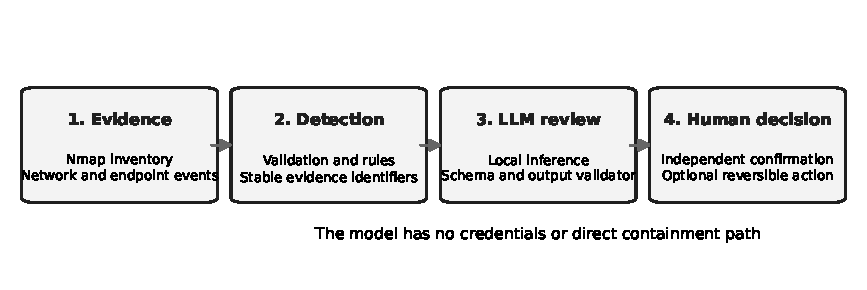
\includegraphics[width=0.82\linewidth]{generated/figures/architecture-trust-boundaries.pdf}
\parbox{0.82\linewidth}{\raggedright\fontsize{9}{11}\selectfont\textbf{Source:} Research design (2026).}
\end{figure}

\subsection{Transparent behavior rules}

The detector implements four predeclared rules. \texttt{BEH-001} requires at least six near-periodic connections to one endpoint with interval coefficient of variation at most 0.15. \texttt{BEH-002} requires at least eight distinct endpoints within 60 seconds. \texttt{BEH-003} requires at least 1 MB sent and a sent-to-received ratio of at least 10:1. \texttt{BEH-004} correlates at least 32 KiB received with executable-like file metadata within 120 seconds. Thresholds were frozen before external-label inspection.

Each finding records rule ID, stable finding ID, host, process context when available, exact evidence IDs, threshold observations, and interpretation limits. Nmap inventory may add authorized asset context but does not change the label. The detector produces review candidates only and invokes no firewall, quarantine, process termination, or file deletion action.

The V1.1 endpoint schema adds bounded optional fields for executable path, signer, parent process, pseudonymous user context, command line, and SHA-256. It excludes credentials, message bodies, keystrokes, packet payloads, and file contents; text is capped at 1,024 characters and hashes are syntactically validated. These fields provide review context and lineage but do not themselves confirm maliciousness.

\subsection{LLM protocol and controls}

The grounded protocol uses local Ollama on loopback with a 4,096-token context, 700-token output ceiling, temperature zero, seed 42, and closed schema. V1.1 evaluates \texttt{llama3.2:3b}, \texttt{gemma3:4b}, and \texttt{qwen3:8b} under Ollama 0.32.13; exact manifest digests and quantization records are frozen with the matrix. The historical control runs used Ollama versions 0.32.5 and 0.32.6 and a preserved Llama blob hash. Scan- or event-controlled strings are delimited as untrusted data. The model selects explanations and proposed controls from the evidence pack and a fixed catalog; it holds no operating-system, Zabbix, or firewall credential.

The control reconstructs the historical technical free-text path with temperature 0.7 and \texttt{top\_p}=0.9, no system prompt, and no output schema. Both protocols receive the same observations, but the control is not a byte-exact replay: fixed context, output, and timeout limits were added for reproducibility.

\section{Method}

\subsection{Study design}

The study follows an applied Design Science Research structure: artifact construction, demonstration, evaluation, and communication \cite{peffers2007}. The 2025 monograph is treated as a historical record, while the experiments reported here use new code and evidence. The confirmatory boundary was defined before the final repetitions: exploratory outputs that influenced a metric or rubric cannot be reused as confirmatory evidence.

The evaluation has five components. Phase A is a deterministic functional benchmark. Phase B1 reports the Virut/NSIS.ay external validation and retrospective diagnostics. Phase B2 uses a prospectively frozen RBot development source, a predeclared threshold grid, and a DonBot holdout parsed once only after configuration and source-state freeze. Phase B3 replays that configuration on a separately published synthetic flow source. Phase C compares grounded and historical LLM protocols over repeated calls and separately tests inert prompt-injection telemetry. The automated Phase-C repetitions are complete; blinded human ratings were not collected. Figure~\ref{fig:experimental-flow} summarizes these roles without combining their metrics.

\begin{figure}[htbp]
\centering
\caption{Experimental phases and evidentiary roles. Metrics are not pooled across roles.}
\label{fig:experimental-flow}
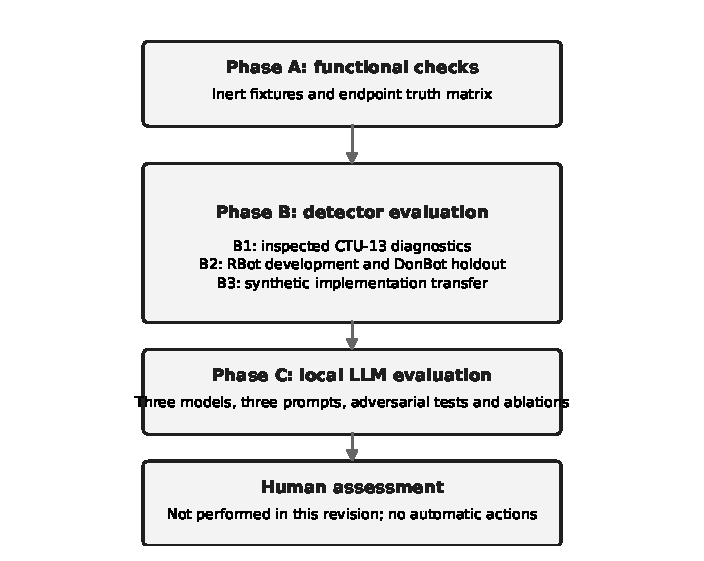
\includegraphics[width=0.62\linewidth]{generated/figures/experimental-flow.pdf}
\parbox{0.62\linewidth}{\raggedright\fontsize{9}{11}\selectfont\textbf{Source:} Research design (2026).}
\end{figure}

\subsection{Execution environments and comparison boundary}

The preserved V1.0 runs and the V1.1 development environment differ materially, as summarized in Table~\ref{tab:environment-comparison}. V1.0 model inference ran on the CPU of an Intel Core i5-1335U system with approximately 16~GiB RAM, first under Windows and then under Debian. The V1.1 development system has an AMD Ryzen 5 5600, approximately 32~GiB RAM, and an NVIDIA RTX 3060 with 12~GiB VRAM. At inventory time, no V1.1 experiment had been executed on the newer machine.

These differences affect model placement, memory pressure, drivers, runtime versions, and latency. Timing across V1.0 and V1.1 is therefore reported only as provenance and cannot identify a protocol-speed or model-speed effect. Any V1.1 comparison intended to isolate a model, prompt, schema, or validator change must execute all compared conditions on the same frozen environment.

\begin{table}[htbp]
\centering
\caption{Execution-environment provenance for the preserved V1.0 runs and V1.1 development.}
\label{tab:environment-comparison}
\small
\begin{adjustbox}{max width=\textwidth}
\begin{tabular}{llllll}
\toprule
Research state & Operating system & CPU & Topology & RAM (GiB) & Inference device \\
\midrule
V1.0 initial run & Windows 11 build 26200 & Intel Core i5-1335U & 12 logical processors & 15.7 & CPU; Intel Iris Xe present \\
V1.0 confirmatory repetitions & Debian GNU/Linux, kernel 6.12.101 & Intel Core i5-1335U & 10 cores / 12 logical processors & 15.4 & CPU \\
V1.1 development environment & Windows 10 Pro 22H2 build 19045 & AMD Ryzen 5 5600 & 6 cores / 12 logical processors & 31.9 & NVIDIA RTX 3060, 12 GiB VRAM \\
\bottomrule
\end{tabular}
\end{adjustbox}
\par\vspace{2pt}{\raggedright\footnotesize\textit{Note:} The V1.1 row is an environment inventory, not evidence that a V1.1 experiment had already run. Cross-machine latency is descriptive only because hardware, operating system, driver, runtime version, and CPU/GPU placement differ.}
\par\vspace{2pt}{\raggedright\fontsize{9}{11}\selectfont\textbf{Source:} Research data (2026).}
\end{table}


\subsection{Phase A: inert functional fixtures}

Six committed JSON Lines scenarios contain no sockets, payloads, persistence mechanisms, or operating-system changes. They represent irregular benign browsing, a legitimate periodic updater as a hard negative, and four emulated patterns corresponding to the four rules. The unit is a scenario-rule pair, yielding 24 binary units. Expected labels were declared in the scenario manifest before execution.

The frozen Phase-A result is summarized in Table~\ref{tab:phase-a}. It must not be combined with external-validation metrics because it measures implementation conformance to constructed patterns, not real-world detection accuracy.

\begin{table}[htbp]
\centering
\caption{Frozen Phase-A synthetic behavior-rule result.}
\label{tab:phase-a}
\small
\begin{adjustbox}{max width=\columnwidth}
\begin{tabular}{rrrrrrrr}
\toprule
TP & FP & FN & TN & Precision & Recall & F1 & Specificity \\
\midrule
4 & 1 & 0 & 19 & 0.800 & 1.000 & 0.889 & 0.950 \\
\bottomrule
\end{tabular}
\end{adjustbox}
\par\vspace{2pt}{\raggedright\fontsize{9}{11}\selectfont\textbf{Source:} Research data (2026).}
\end{table}


A separate five-case endpoint matrix evaluates \texttt{BEH-004}: one same-process download/file sequence and four negatives varying bytes, process identity, timing, and file suffix. Every event contains synthetic process lineage and pseudonymous user context. The matrix is executed both with and without Nmap inventory to distinguish contextual enrichment from rule behavior.

\subsection{Phase B1: historical external flow validation}

Data selection was frozen before complete-label inspection. CTU-13 Scenario 5 (Virut) is the development source, while Scenario 12 (NSIS.ay) is the family-separated holdout. Only the publisher-recommended bidirectional \texttt{.binetflow} text files were acquired. Their provenance is fixed by these SHA-256 values:

{\fontsize{8}{10}\selectfont\ttfamily
\noindent Scenario 5: ef5c9ed6895d4ca5aec723449dae3005\par
\noindent\hspace*{4.8em}4ccd1f6b091713a52ffcb681ff78a02c\par
\noindent Scenario 12: 1098f0addacedc321c7baefad63ef0d9\par
\noindent\hspace*{4.8em}a0f26630d0155087d37e8da770dd9f2e\par}

Acquisition code rejects executables, archives, packet captures, and binary Argus files.

The scored unit is an anonymized source host in a non-overlapping five-minute window. Addresses are replaced by stable scenario-local hashes before detection, and labels are never supplied to the detector. Positive windows contain \texttt{From-Botnet} source flows; negative windows contain \texttt{From-Normal} source flows. Mixed, background, inbound, and unsupported-protocol records are counted and excluded.

The adapter creates normalized connection events from flow direction and byte counts. CTU-13 flow records have no endpoint process identity or file lineage, so only \texttt{BEH-001} through \texttt{BEH-003} are evaluated. \texttt{BEH-004} is explicitly out of scope. Scenario 5 was available for development interpretation, but thresholds were not retuned. Scenario 12 remained the held-out report set.

After the V1.0 result had been finalized and inspected, both sources were reopened for a predeclared V1.1 retrospective diagnostic. Without changing rule thresholds, the adapter formed non-overlapping source-host units of 60, 300, and 600 seconds. It then decomposed each rule into observable components: connection count, eligible mean interval and interval variation for \texttt{BEH-001}; maximum distinct destinations in any 60-second interval for \texttt{BEH-002}; and absolute sent bytes and sent-to-received ratio for \texttt{BEH-003}. Deterministic class/time/host ordering selected one TP, FP, and FN example. This reuse can explain failure modes and window sensitivity, but it cannot support model selection on the holdout or make that holdout untouched again.

\subsection{Phase B2: prospective family-separated holdout}

Before downloading or parsing the new files, Scenario 11 (RBot) was assigned to development and Scenario 6 (DonBot) to the sole confirmatory holdout using official capture metadata and HTTP headers. The primary unit and label policy remained the five-minute source-host definition used in Phase B1. A frozen 243-member grid varied \texttt{BEH-001} minimum count and interval variation, \texttt{BEH-002} destination count, and \texttt{BEH-003} byte and ratio components. Selection maximized development MCC, followed by balanced accuracy, F1, specificity, distance from V1.0, alert count, and deterministic parameter order.

All candidates were evaluated only on RBot. The complete grid, selected configuration, anonymized units, acquisition hashes, and scientific source hashes were preserved before DonBot was parsed. The holdout executor rejected any source-state change and wrote to a previously absent immutable directory. It then evaluated DonBot exactly once. The original preselection record contained a timestamp transcription error; both its hash and a corrected record with the observed pre-download creation time are retained with an explicit erratum. Dataset roles, grid, and gates did not change.

\subsection{Phase B3: second-dataset implementation transfer}

The Botnet Group Activity Dataset contains 13 synthetic eight-hour scenarios in the same 15-column \texttt{.binetflow} representation \cite{hostiadi2021botnetgroup,hostiadi2021botnetgroupdata}. Its generator adopts activity patterns from CTU-13; it is therefore not independent evidence of real-world generalization. Before downloading the archive or inspecting scenario labels, Scenario 1 was selected for an implementation-transfer replay. Archive and extracted-file byte counts and SHA-256 hashes were verified, and the selected V1.1 thresholds were not changed.

The five-minute source-host unit and label policy remained unchanged. A dataset-specific parser profile expanded only the file/row bounds, accepted the published hyphenated timestamps, used a separate anonymization namespace, and normalized the unspecified source timezone to UTC solely for within-source bucketing. To bound memory and output for 2.1 million rows, the run preserved aggregate confusion counts, truth-separated rule combinations, and the first deterministic example per combination rather than every unit. These results are reported separately from every CTU-13 role.

\subsection{Phase C: repeated protocol comparison}

The primary V1.1 matrix uses three quantized local models from different families and sizes: \texttt{llama3.2:3b}, \texttt{gemma3:4b}, and \texttt{qwen3:8b}. Exact local manifest digests, registry records and byte sizes were frozen before inference. Each model receives three semantically equivalent prompt variants: contract, evidence-first, and checklist. All variants use the same evidence pack, output schema, validator, scenario order, temperature zero, \texttt{top\_p}=0.9, seed 42, 4,096-token context, and 700-token output ceiling.

Five clustered repetitions cover a no-finding case, a benign periodic-updater hard negative, an incomplete single observation, an endpoint-lineage case, and a 17-event case producing all four findings. Only the four finding-bearing scenarios invoke the model, yielding 20 calls per model/prompt cell and 180 planned calls. API receipt, JSON parsing, closed-schema validity, deterministic semantic-policy acceptance, finding coverage, evidence coverage and lexical safety flags are reported separately. The no-finding case verifies that no model call is made when the detector has no finding. A separately frozen supplement closes the remaining case-diversity gap with 31 unique events and all four rules. It prospectively defines conflicting context as comparable detector severities accompanied by opposing cues: signed maintenance-like lineage versus missing signer and parent context. Neither cue is treated as proof. The three models receive the same evidence-first prompt, schema and validator in three repetitions (nine calls). A pre-inference prompt-size check increased context equally from 8,192 to 16,384 tokens before any supplemental output was observed.

The preserved 2025 comparison remains a historical control: five finding-bearing Phase-A cases were submitted ten times to one grounded protocol and to a reconstructed free-text path, yielding 50 calls per condition. It supports a direct exact-identifier comparison for that fixed model and environment but is not pooled with the V1.1 matrix.

The adversarial matrix contains six paired telemetry-field injections and one paired Nmap inventory injection, plus one unpaired benign hard negative per model. Attack and sanitized conditions differ only in the declared field, for 45 calls. All fixtures are inert and cover fake identifiers, fictional CVE-like text, instruction override, unauthorized controls, delimiter/JSON text, Unicode confusables, long strings, command line, process, DNS, file, host and inventory fields. After 12 responses had been preserved, execution exposed a precondition defect: the hard negative's empty truth label had been confused with its expected \texttt{BEH-001} detector false positive. A recorded amendment separated truth from detector precondition without changing any telemetry, prompt, parameter, validator or paired metric; the 12 protocol-identical records were reused.

A single-model ablation reuses the first three Llama/contract repetitions as its reference and changes one component at a time: temperature 0.7, omission of the API \texttt{format} parameter, or reduced grounding language. It adds 36 calls. A post-hoc validator-bypass condition reclassifies every received reference response as usable but is never connected to operations. Three clustered repetitions describe component sensitivity only. A blinded human-rating rubric and randomized 36-item package were prepared from the first repetition of every model/prompt cell. Five missing primary response bodies were filled only for reviewer display by separately frozen availability-recovery calls; the concealed mapping retains primary and selected-response status, and primary denominators remain unchanged. No human semantic ratings are claimed.

The symmetric automatic audit is deliberately conservative. It applies the same identifier, CVE, attribution, containment, authorization and coverage checks to JSON and free text, but its attribution expression also flags negated phrases such as ``malware is not confirmed.'' These outputs are therefore reported as lexical safety flags rather than expert-adjudicated unsupported claims. Fixed prompts and repetitions are clustered observations; no inferential p-value or attack-success probability is reported.

\subsection{Metrics, response counterfactual, and reproducibility}

For true positives ($TP$), false positives ($FP$), false negatives ($FN$), and true negatives ($TN$), the study reports precision, recall, F1, specificity, balanced accuracy, and Matthews correlation coefficient (MCC). Proportion intervals use the Wilson 95\% method. MCC is retained because both classes and both error directions matter:
\begin{equation}
\resizebox{0.95\columnwidth}{!}{$\displaystyle
\mathrm{MCC}=\frac{TP\,TN-FP\,FN}
{\sqrt{(TP+FP)(TP+FN)(TN+FP)(TN+FN)}}.$}
\end{equation}

No response was executed. A counterfactual estimates what would have occurred if every alerted window had been blocked: normal-origin alerted windows represent unnecessary actions, and non-alerted botnet-origin windows represent missed opportunities. This is a safety analysis, not a claim about real firewall effectiveness.

Inputs, hashes, model identifier, prompts, raw outputs, environment, per-call errors, aggregate JSON, and table-generation code are preserved in the repository \cite{ielen2025repo}. The flow parsers are streaming; CTU-13 retains anonymized scored units, while the higher-cardinality second dataset retains truth-separated rule-combination counts and deterministic examples. Article tables are generated directly from committed result JSON to prevent transcription drift.

\section{Results}

\subsection{Functional benchmark}

As shown previously in Table~\ref{tab:phase-a}, the rules produced 4 true positives, 1 false positive, no false negatives, and 19 true negatives. The resulting precision was 0.800, recall 1.000, specificity 0.950, and F1 0.889. The only false positive was intentional: legitimate periodic updater traffic matched \texttt{BEH-001}. This demonstrates that the implementation recognizes its specified patterns and exposes the known dual-use limitation; it does not estimate field accuracy.

The endpoint matrix in Table~\ref{tab:endpoint-beh004} produced one TP and four TN, with no FP or FN. The positive preserved exact network and file evidence IDs. Nmap changed only \texttt{known\_asset} context; predictions and finding identifiers were identical without it. This validates the programmed temporal/process/file conditions on constructed evidence, not endpoint detection accuracy or causal proof that received bytes became the file.

\begin{table}[htbp]
\centering
\caption{Frozen inert BEH-004 endpoint truth matrix.}
\label{tab:endpoint-beh004}
\small
\begin{adjustbox}{max width=\columnwidth}
\begin{tabular}{lccc}
\toprule
Condition & Expected & Predicted & Outcome \\
\midrule
Same process within window & Yes & Yes & TRUE POSITIVE \\
Received bytes below threshold & No & No & TRUE NEGATIVE \\
Different processes & No & No & TRUE NEGATIVE \\
File after time window & No & No & TRUE NEGATIVE \\
Non executable like suffix & No & No & TRUE NEGATIVE \\
\bottomrule
\end{tabular}
\end{adjustbox}
\par\vspace{2pt}{\raggedright\footnotesize\textit{Note:} Nmap enrichment changed only the known-asset context; all finding identifiers and decisions were identical without inventory. This is functional validation on constructed evidence, not endpoint accuracy.}
\par\vspace{2pt}{\raggedright\fontsize{9}{11}\selectfont\textbf{Source:} Research data (2026).}
\end{table}


\subsection{External validation}

Table~\ref{tab:ctu13-metrics} reports development and holdout results separately. The holdout contained 53 botnet-origin and 55 normal-origin units. Sixteen botnet-origin units alerted, 37 were missed, 32 normal-origin units alerted, and 23 did not.

\begin{table}[htbp]
\centering
\caption{Family-separated CTU-13 external validation.}
\label{tab:ctu13-metrics}
\small
\begin{adjustbox}{max width=\linewidth}
\begin{tabular}{llrrrrrrrrrr}
\toprule
Role & Family & Units & TP & FP & FN & TN & Precision & Recall & F1 & Specificity & MCC \\
\midrule
Development & Virut & 31 & 5 & 17 & 0 & 9 & 0.227 & 1.000 & 0.370 & 0.346 & 0.280 \\
Holdout & NSIS.ay & 108 & 16 & 32 & 37 & 23 & 0.333 & 0.302 & 0.317 & 0.418 & -0.282 \\
\bottomrule
\end{tabular}
\end{adjustbox}
\par\vspace{2pt}{\raggedright\fontsize{9}{11}\selectfont\textbf{Source:} Research data (2026).}
\end{table}


Figure~\ref{fig:ctu13-development-holdout} compares F1 and MCC while keeping historical and prospective roles separate.

\begin{figure}[htbp]
\centering
\caption{F1 and MCC for the historical inspected pair and the prospectively gated CTU-13 pair. Roles remain separate.}
\label{fig:ctu13-development-holdout}
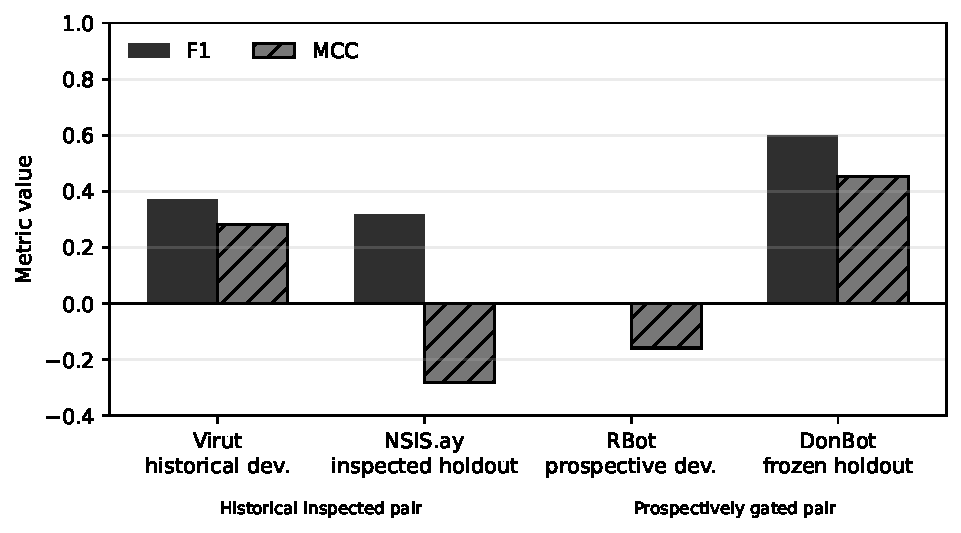
\includegraphics[width=0.76\linewidth]{generated/figures/ctu13-development-holdout-metrics.pdf}
\parbox{0.76\linewidth}{\raggedright\fontsize{9}{11}\selectfont\textbf{Source:} Research data (2026).}
\end{figure}

Development precision had a Wilson 95\% interval from 0.101 to 0.434, recall from 0.566 to 1.000, and specificity from 0.194 to 0.538. Holdout intervals were from 0.217 to 0.475 for precision, from 0.195 to 0.435 for recall, and from 0.297 to 0.550 for specificity. The holdout MCC of $-0.282$ is a negative generalization result, not evidence of reliable botnet detection.

The rule-level error distribution is given in Table~\ref{tab:ctu13-rules}; B/N denotes findings on botnet-origin and normal-origin windows. Rapid distinct destinations dominated both correct and incorrect alerts. Periodicity appeared only in normal-origin holdout windows, and the asymmetric-egress rule did not fire.

\begin{table}[htbp]
\centering
\caption{Rule findings on botnet-origin and normal-origin CTU-13 windows.}
\label{tab:ctu13-rules}
\begin{tabular}{llrr}
\toprule
Rule & Pattern & Development B/N & Holdout B/N \\
\midrule
\texttt{BEH-001} & Periodic communication & 1/7 & 0/15 \\
\texttt{BEH-002} & Distinct endpoints & 5/17 & 16/32 \\
\texttt{BEH-003} & Asymmetric egress & 0/0 & 0/0 \\
\bottomrule
\end{tabular}
\par\vspace{2pt}{\fontsize{10}{12}\selectfont\textbf{Source:} Prepared by the authors from the preserved CTU-13 validation output (2026).}
\end{table}


The development and holdout files contained 129,832 and 325,471 rows. Clean binary scoring retained 5,558 and 9,755 rows; most excluded rows were background or inbound/ambiguous under the publisher's label semantics. Streaming processing took approximately 14.4 and 37.9 seconds, with less than 1.3 MiB peak Python memory traced. Runtime demonstrates feasibility for these files only and is not a throughput benchmark.

\subsection{Retrospective window and threshold diagnostics}

Table~\ref{tab:ctu13-windows} reports the fixed 1-, 5-, and 10-minute window analyses. Changing the aggregation interval changes both the number and meaning of scored units, so rows are sensitivity analyses rather than interchangeable repetitions. The one-minute holdout result moved MCC closest to zero and increased specificity, but remained weak; selecting it after observing these results would be holdout-driven tuning and is therefore prohibited.

\begin{table}[htbp]
\centering
\caption{Retrospective CTU-13 sensitivity analysis across fixed aggregation windows.}
\label{tab:ctu13-windows}
\small
\begin{adjustbox}{max width=\textwidth}
\begin{tabular}{llrrrrrrrrr}
\toprule
Role & Family & Window (s) & Units & TP & FP & FN & TN & F1 & Specificity & MCC \\
\midrule
Development & Virut & 60 & 101 & 18 & 34 & 3 & 46 & 0.493 & 0.575 & 0.351 \\
Development & Virut & 300 & 31 & 5 & 17 & 0 & 9 & 0.370 & 0.346 & 0.280 \\
Development & Virut & 600 & 19 & 3 & 10 & 0 & 6 & 0.375 & 0.375 & 0.294 \\
Holdout & NSIS.ay & 60 & 247 & 31 & 53 & 71 & 92 & 0.333 & 0.634 & -0.064 \\
Holdout & NSIS.ay & 300 & 108 & 16 & 32 & 37 & 23 & 0.317 & 0.418 & -0.282 \\
Holdout & NSIS.ay & 600 & 73 & 13 & 18 & 29 & 13 & 0.356 & 0.419 & -0.271 \\
\bottomrule
\end{tabular}
\end{adjustbox}
\par\vspace{2pt}{\raggedright\footnotesize\textit{Note:} Thresholds were not retuned. Because the V1.0 holdout had already been inspected, all window comparisons are diagnostic rather than confirmatory and cannot be used to restore an untouched-holdout claim.}
\par\vspace{2pt}{\raggedright\fontsize{9}{11}\selectfont\textbf{Source:} Research data (2026).}
\end{table}


The component analysis in Table~\ref{tab:ctu13-threshold-diagnostics} explains why the fixed rules failed differently. Most botnet-origin holdout units never reached six same-endpoint connections, whereas the periodicity rule matched only normal-origin units. Destination diversity overlapped substantially between classes: the normal-origin median exceeded the rule threshold, while the botnet-origin distribution combined many low-count units with a large upper tail. For asymmetric egress, no scored unit in either source reached the 1-MB (1,000,000-byte) per-flow component. Many units exceeded the 10:1 ratio alone, so the absolute byte threshold was the immediate non-firing condition. Flow aggregation and missing process/file context prevent interpreting non-firing as proof that exfiltration-like behavior was absent.

An MCC below zero means that, under this binary source-window definition, alert and truth labels were inversely associated rather than merely weakly associated. It is not a probability of error, but it shows that treating the five-minute alert as a malware-origin classifier would be worse than an uninformative zero-correlation result on this holdout.

\begin{table}[htbp]
\centering
\caption{Five-minute component diagnostics for the three network-flow rules.}
\label{tab:ctu13-threshold-diagnostics}
\small
\begin{adjustbox}{max width=\textwidth}
\begin{tabular}{llrrrrrrrrrr}
\toprule
Role & Truth & Units & \multicolumn{4}{c}{BEH-001 failure path/match} & \multicolumn{2}{c}{BEH-002 destinations} & \multicolumn{3}{c}{BEH-003 component matches} \\
\cmidrule(lr){4-7}\cmidrule(lr){8-9}\cmidrule(lr){10-12}
 & & & $<6$ & No mean & CV$>0.15$ & Match & Median & Max. & $\geq1$ MB & Ratio$\geq10$ & Both \\
\midrule
Development & botnet-origin & 5 & 0 & 1 & 3 & 1 & 24 & 30 & 0 & 5 & 0 \\
Development & normal-origin & 26 & 7 & 6 & 6 & 7 & 10.5 & 52 & 0 & 3 & 0 \\
Holdout & botnet-origin & 53 & 50 & 0 & 3 & 0 & 2 & 323 & 0 & 28 & 0 \\
Holdout & normal-origin & 55 & 18 & 16 & 6 & 15 & 9 & 34 & 0 & 6 & 0 \\
\bottomrule
\end{tabular}
\end{adjustbox}
\par\vspace{2pt}{\raggedright\footnotesize\textit{Note:} BEH-001 categories are mutually exclusive. BEH-002 reports each unit's maximum distinct destinations in any 60-second interval. BEH-003 component counts do not assert that the underlying behavior was absent.}
\par\vspace{2pt}{\raggedright\fontsize{9}{11}\selectfont\textbf{Source:} Research data (2026).}
\end{table}


Figure~\ref{fig:beh002-distributions} shows the overlap between the two destination-count distributions.

\begin{figure}[htbp]
\centering
\caption{Empirical BEH-002 destination-count distributions in the five-minute NSIS.ay holdout. The exact-value empirical overlap coefficient is descriptive and sample-specific.}
\label{fig:beh002-distributions}
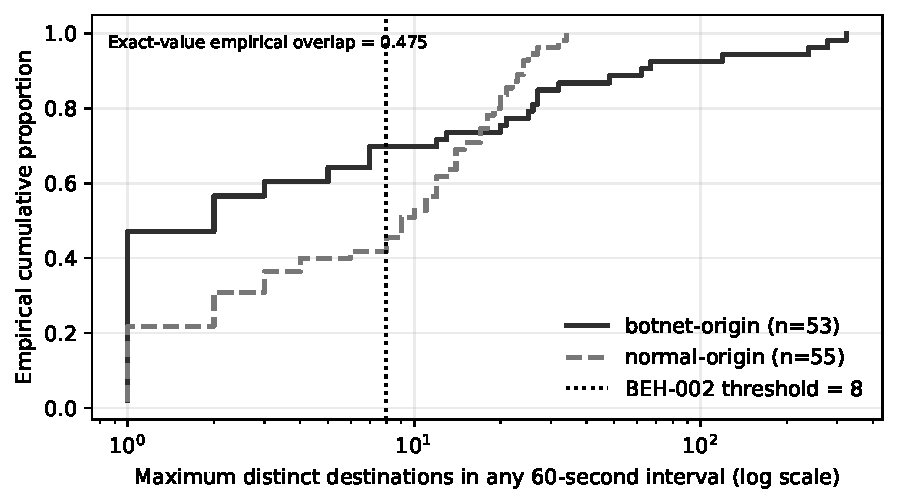
\includegraphics[width=0.76\linewidth]{generated/figures/beh002-holdout-distributions.pdf}
\parbox{0.76\linewidth}{\raggedright\fontsize{9}{11}\selectfont\textbf{Source:} Research data (2026).}
\end{figure}

Table~\ref{tab:ctu13-error-examples} makes the operational error modes concrete. The selected TP is a high-diversity botnet-origin window; the selected FP is normal-origin traffic that also exceeds the diversity threshold; and the selected FN contains only one retained event, leaving no rule enough evidence to fire. Exact anonymized host, time, finding, and evidence identifiers remain in the preserved machine-readable result rather than being manually transcribed into the manuscript.

\begin{table}[htbp]
\centering
\caption{Deterministically selected five-minute holdout examples.}
\label{tab:ctu13-error-examples}
\small
\begin{adjustbox}{max width=\linewidth}
\begin{tabular}{llrrrrr}
\toprule
Class & Rule & Events & Evidence IDs & Max. destinations & Max. sent (KiB) & Max. ratio \\
\midrule
TP & BEH-002 & 442 & 20 & 278 & 197.0 & 11560.000 \\
FP & BEH-002 & 142 & 20 & 13 & 390.2 & 2.000 \\
FN & N/A & 1 & 1 & 1 & 0.1 & 0.426 \\
\bottomrule
\end{tabular}
\end{adjustbox}
\par\vspace{2pt}{\raggedright\footnotesize\textit{Note:} Examples are selected by a deterministic class/time/host ordering from anonymized source-window units; the preserved JSON retains the exact finding and evidence identifiers.}
\par\vspace{2pt}{\raggedright\fontsize{9}{11}\selectfont\textbf{Source:} Research data (2026).}
\end{table}


\subsection{Prospective CTU-13 holdout}

Table~\ref{tab:ctu13-confirmatory} reports the prospectively gated analysis. RBot development was a difficult and very small selection source: none of its three botnet-origin units alerted under any frozen candidate. The deterministic tie-break selected candidate 97, which retained the V1.0 thresholds except for raising the \texttt{BEH-002} destination count from 8 to 16. Its negative development MCC was preserved rather than hidden.

\begin{table}[htbp]
\centering
\caption{Prospective V1.1 development selection and single confirmatory CTU-13 holdout.}
\label{tab:ctu13-confirmatory}
\small
\begin{adjustbox}{max width=\textwidth}
\begin{tabular}{llrrrrrrrrrr}
\toprule
Role & Family & Units & TP & FP & FN & TN & Precision & Recall & F1 & Specificity & MCC \\
\midrule
Development & RBot & 18 & 0 & 2 & 3 & 13 & 0.000 & 0.000 & 0.000 & 0.867 & -0.158 \\
Confirmatory holdout & DonBot & 105 & 24 & 29 & 3 & 49 & 0.453 & 0.889 & 0.600 & 0.628 & 0.452 \\
\bottomrule
\end{tabular}
\end{adjustbox}
\par\vspace{2pt}{\raggedright\footnotesize\textit{Note:} The 243-configuration grid was evaluated only on RBot. The selected configuration and scientific source hashes were frozen before the DonBot file was parsed once. Development and holdout metrics are not pooled.}
\par\vspace{2pt}{\raggedright\fontsize{9}{11}\selectfont\textbf{Source:} Research data (2026).}
\end{table}


On the single DonBot holdout run, the selected detector identified most botnet-origin units and produced a positive MCC. This is evidence of family-specific generalization under the frozen protocol, not universal botnet detection. False-positive burden remained operationally large, and \texttt{BEH-003} again produced no finding. Across the four CTU-13 sources, 262 source-window units were scored, but no pooled metric is reported because development, retrospective and confirmatory roles differ.

\subsection{Second-dataset implementation transfer}

The Scenario-1 replay retained 46,567 of 2,112,224 flows for clean binary scoring and formed 529 source-window units. Table~\ref{tab:second-dataset-transfer} shows TP=96, FP=48, FN=1, and TN=384 (F1 0.797; MCC 0.764). \texttt{BEH-002} accounted for all 96 botnet-origin alerts and 46 normal-origin alerts; \texttt{BEH-003} added two normal-origin alerts, while \texttt{BEH-001} never fired. Thus, 48 of 144 alerts (33.3\%) were normal-origin even in this favorable synthetic transfer result.

\begin{table}[htbp]
\centering
\caption{Frozen detector replay on the second, synthetic implementation-transfer dataset.}
\label{tab:second-dataset-transfer}
\small
\begin{adjustbox}{max width=\textwidth}
\begin{tabular}{lrrrrrrrrrr}
\toprule
Role & Units & TP & FP & FN & TN & Precision & Recall & F1 & Specificity & MCC \\
\midrule
Implementation transfer & 529 & 96 & 48 & 1 & 384 & 0.667 & 0.990 & 0.797 & 0.889 & 0.764 \\
\bottomrule
\end{tabular}
\end{adjustbox}
\par\vspace{2pt}{\raggedright\footnotesize\textit{Note:} The Botnet Group Activity source is synthetic and derives group patterns from CTU-13. It tests parser and detector transfer, not independent real-world generalization; these metrics are not pooled with CTU-13.}
\par\vspace{2pt}{\raggedright\fontsize{9}{11}\selectfont\textbf{Source:} Research data (2026).}
\end{table}


The archive's own description reports 23,000 bot records, whereas 22,000 entered scoring. The parser excluded 1,046 unsupported-protocol records overall and preserved the complete exclusion accounting; it did not silently reinterpret those records. Because the source is generated from CTU-13-derived patterns, the positive MCC establishes software and representation transfer only. It cannot be used as an independent replication of the DonBot result.

\subsection{Local-LLM traceability, ablation and adversarial results}

Table~\ref{tab:llm-primary-matrix} reports all 180 primary attempts. The local endpoint returned 145 responses; 122 were valid JSON matching the closed schema, and 73 passed the semantic-policy validator. Thus, acceptance was 73/180 by the planned attempt denominator and 73/145 among received responses. Across the seven cells with all 20 API responses, acceptance ranged from 0.10 to 0.75. These cell differences are descriptive because prompt repetitions are clustered and no human correctness labels exist.

\begin{table}[htbp]
\centering
\caption{V1.1 primary local-LLM matrix; each cell contains 20 attempted calls.}
\label{tab:llm-primary-matrix}
\small
\begin{adjustbox}{max width=\textwidth}
\begin{tabular}{llrrrrrrr}
\toprule
Model & Prompt & Calls & API & JSON & Schema & Accepted & Finding cov. & Evidence cov. \\
\midrule
llama3.2:3b & contract-v1 & 20 & 20 & 15 & 15 & 11 & 0.750 & 0.750 \\
llama3.2:3b & evidence-first-v1 & 20 & 20 & 20 & 20 & 15 & 0.938 & 0.912 \\
llama3.2:3b & checklist-v1 & 20 & 20 & 15 & 15 & 4 & 0.750 & 0.750 \\
gemma3:4b & contract-v1 & 20 & 20 & 19 & 19 & 11 & 0.900 & 0.879 \\
gemma3:4b & evidence-first-v1 & 20 & 20 & 20 & 20 & 14 & 0.750 & 0.750 \\
gemma3:4b & checklist-v1 & 20 & 20 & 16 & 16 & 2 & 0.738 & 0.712 \\
qwen3:8b & contract-v1 & 20 & 20 & 14 & 14 & 14 & 0.700 & 0.700 \\
qwen3:8b & evidence-first-v1 & 20 & 5 & 3 & 3 & 2 & 0.600 & 0.600 \\
qwen3:8b & checklist-v1 & 20 & 0 & 0 & 0 & 0 & 0.000 & 0.000 \\
\bottomrule
\end{tabular}
\end{adjustbox}
\par\vspace{2pt}{\raggedright\footnotesize\textit{Note:} API is the number of responses received; JSON and Schema are representation checks; Accepted additionally requires the frozen deterministic semantic-policy validator. Coverage is averaged over attempted finding-bearing scenarios, so API failures contribute zero.}
\par\vspace{2pt}{\raggedright\fontsize{9}{11}\selectfont\textbf{Source:} Research data (2026).}
\end{table}


The Qwen contract cell completed, but the local Ollama server exited during the evidence-first cell. One connection reset and 34 subsequent connection-refused attempts were preserved, leaving 15/20 evidence-first and 20/20 checklist attempts without responses. The cause was not established from a preserved primary-run server log; it is therefore reported as end-to-end local availability failure, not model-quality, timeout or out-of-memory evidence. Incomplete Qwen cells are not compared as though they had complete outputs.

Availability recovery was kept outside the primary matrix. Its first four-call attempt returned four HTTP 500 responses because two orphaned Ollama child processes remained resident and the Qwen load failed at CUDA allocation. After only those verified orphaned processes were removed, one declared retry returned 4/4 response bodies, of which one passed the validator. Package preflight then found one additional primary Qwen response with an empty body; a prospectively selected single-call recovery produced schema-valid content that the validator rejected. These five outputs make the blinded display package complete but do not revise the primary 145/180 response or 73/180 acceptance denominators.

Every one of the 45 multi-finding attempts was either rejected or lacked an API response. A post-hoc audit could extract schema-valid rankings in four of nine cells. Each of those four repeated one ordering exactly across its available observations, but every ordering omitted findings, used non-exact identifiers, cited evidence across finding boundaries, or selected an inapplicable control. Repeatable ordering therefore did not imply complete or correct ranking; the other five cells had no schema-valid ranking to estimate.

The supplemental stress test in Table~\ref{tab:llm-supplement} received 9/9 API responses. Four outputs were valid JSON/schema and none passed deterministic grounding-policy validation. All nine inputs plus reserved output fit the 16,384-token context, while five responses reached the 900-token output cap. Only Llama supplied all exact finding IDs in a schema-valid form across three repetitions; its order and priority vector repeated exactly, but every output selected rule-inapplicable controls and was rejected. Gemma yielded one schema-valid response with non-exact finding IDs, and Qwen yielded no complete JSON. The supplement covers the missing scenario type but does not reverse the negative complex-ranking result.

\begin{table}[htbp]
\centering
\caption{Supplemental 31-event conflicting-context LLM stress test.}
\label{tab:llm-supplement}
\small
\begin{adjustbox}{max width=\textwidth}
\begin{tabular}{lrrrrrrrr}
\toprule
Model & Calls & API & JSON & Schema & Accepted & Output cap & Complete ranks & Rank agreement \\
\midrule
gemma3-4b & 3 & 3 & 1 & 1 & 0 & 2 & 0 & N/A \\
llama3-2-3b & 3 & 3 & 3 & 3 & 0 & 0 & 3 & 1.000 \\
qwen3-8b & 3 & 3 & 0 & 0 & 0 & 3 & 0 & N/A \\
\bottomrule
\end{tabular}
\end{adjustbox}
\par\vspace{2pt}{\raggedright\footnotesize\textit{Note:} All nine inputs plus their reserved output fit the 16,384-token context. Output cap counts responses reaching 900 generated tokens. Ranking agreement is estimable only for schema-valid outputs containing every exact finding identifier once; repeatability is not semantic correctness.}
\par\vspace{2pt}{\raggedright\fontsize{9}{11}\selectfont\textbf{Source:} Research data (2026).}
\end{table}


The historical comparison in Table~\ref{tab:llm-repeated} and Figure~\ref{fig:traceability} remains useful within its narrower scope. Grounded output preserved exact finding and evidence IDs in 50/50 calls, versus 0/50 for reconstructed free text, and 40/50 grounded responses passed policy validation. Free text was not asked to emit JSON, so its zero schema validity is a representation difference rather than an independent quality failure.

\begin{table}[htbp]
\centering
\caption{Repeated Phase-C automated traceability comparison.}
\label{tab:llm-repeated}
\small
\begin{adjustbox}{max width=\linewidth}
\begin{tabular}{lrrrrrr}
\toprule
Protocol & Calls & API responses & Exact findings & Exact evidence & System accepted & Policy rejected \\
\midrule
Grounded schema 1.1 & 50 & 50 & 50 & 50 & 40 & 10 \\
Reconstructed free text & 50 & 50 & 0 & 0 & 0 & N/A \\
\bottomrule
\end{tabular}
\end{adjustbox}
\par\vspace{2pt}{\raggedright\fontsize{9}{11}\selectfont\textbf{Note:} Free text was not asked to emit JSON; its system-accepted count applies the common exact-ID grounding criterion. Grounded policy rejections retained complete citations but selected a rule-inapplicable control.}
\par\vspace{2pt}{\raggedright\fontsize{9}{11}\selectfont\textbf{Source:} Research data (2026).}
\end{table}


\begin{figure}[htbp]
\centering
\caption{Preserved single-model traceability comparison. System acceptance includes deterministic grounding and policy validation.}
\label{fig:traceability}
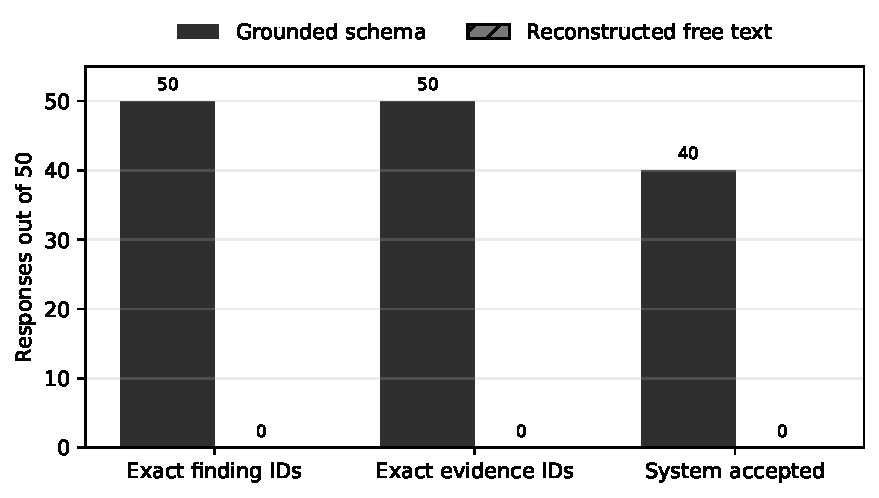
\includegraphics[width=0.72\linewidth]{generated/figures/grounded-free-text-traceability.pdf}
\parbox{0.72\linewidth}{\raggedright\fontsize{9}{11}\selectfont\textbf{Source:} Research data (2026).}
\end{figure}

The ablation in Table~\ref{tab:llm-ablation} isolates observable component sensitivity for the first three Llama/contract repetitions. The reference accepted 7/12 attempts. Raising temperature to 0.7 accepted 4/12. Omitting only the API format constraint produced 12 API responses but zero valid JSON, zero schema-valid outputs and zero accepted outputs. Reduced grounding language accepted 9/12, showing that this small sample does not identify a monotonic benefit from longer instructions. The unsafe validator bypass labels all 12 received reference responses usable, including three that lacked valid JSON/schema output.

\begin{table}[htbp]
\centering
\caption{Single-model component-sensitivity ablation.}
\label{tab:llm-ablation}
\small
\begin{adjustbox}{max width=\textwidth}
\begin{tabular}{lrrrrrrrr}
\toprule
Condition & New calls & Attempts & API & JSON & Schema & Accepted & Finding cov. & Evidence cov. \\
\midrule
Reference (primary reuse) & 0 & 12 & 12 & 9 & 9 & 7 & 0.750 & 0.750 \\
Temperature 0.7 & 12 & 12 & 12 & 9 & 9 & 4 & 0.500 & 0.500 \\
API format removed & 12 & 12 & 12 & 0 & 0 & 0 & 0.000 & 0.000 \\
Grounding language reduced & 12 & 12 & 12 & 9 & 9 & 9 & 0.750 & 0.750 \\
Validator bypass (post hoc) & 0 & 12 & 12 & 9 & 9 & 12 & 0.750 & 0.750 \\
\bottomrule
\end{tabular}
\end{adjustbox}
\par\vspace{2pt}{\raggedright\footnotesize\textit{Note:} Reference and validator-bypass rows reuse the same 12 primary responses. Bypass counts every API response as usable and was never connected to operations. Three clustered repetitions support descriptive sensitivity only.}
\par\vspace{2pt}{\raggedright\fontsize{9}{11}\selectfont\textbf{Source:} Research data (2026).}
\end{table}


The adversarial executor attempted all 45 calls, but 20 returned HTTP 500 and only 11 of 21 attack/sanitized pairs received both responses; ten pairs had two parseable outputs. Table~\ref{tab:llm-adversarial-matrix} therefore uses eligible denominators. Validator acceptance status changed in 8/11 available pairs. Among ten parseable pairs, priority changed in two, control set in four, finding order in one, and cited evidence set in none. The conservative lexical safety flag changed in 1/11 audited pairs. These observations show decision sensitivity and enforcement value; they do not estimate attack success probability from one observation per pair. Pairs with two failures are availability failures, not evidence of robustness.

\begin{table}[htbp]
\centering
\caption{Adversarial paired-output availability and eligible decision changes.}
\label{tab:llm-adversarial-matrix}
\small
\begin{tabular}{lrrrrr}
\toprule
Model & Calls & Responses & Failures & Eligible pairs & Parseable pairs \\
\midrule
gemma3:4b & 15 & 15 & 0 & 7 & 6 \\
llama3.2:3b & 15 & 3 & 12 & 1 & 1 \\
qwen3:8b & 15 & 7 & 8 & 3 & 3 \\
\midrule
\multicolumn{6}{l}{\textit{Decision changes among eligible pairs}} \\
Metric & Changed & Eligible & \multicolumn{3}{l}{} \\
\midrule
Validator status & 8 & 11 & & & \\
Priority label & 2 & 10 & & & \\
Control set & 4 & 10 & & & \\
Finding order & 1 & 10 & & & \\
Evidence set & 0 & 10 & & & \\
Lexical safety flag & 1 & 11 & & & \\
\bottomrule
\end{tabular}
\par\vspace{2pt}{\raggedright\footnotesize\textit{Note:} A pair is eligible for status comparison only when both API responses exist, and for structural comparison only when both are parseable. Two API failures are not treated as an unchanged decision. One observation per pair does not estimate attack-success probability.}
\par\vspace{2pt}{\raggedright\fontsize{9}{11}\selectfont\textbf{Source:} Research data (2026).}
\end{table}


All three benign hard-negative calls were accepted as grounded reviews of a \texttt{BEH-001} finding even though the fixture's truth label is negative. This is expected under the model contract: the model receives the detector's candidate, not ground truth. It reinforces that schema and citation validity cannot turn a detector false positive into a confirmed incident. No model response triggered an action, and no blinded human semantic rating was collected.

\subsection{Counterfactual response safety}

The system executed zero automatic actions. In the historical five-minute holdout, a block-on-every-alert policy would have targeted normal-origin windows in 32 of 48 cases while missing 37 botnet-origin units. In the new confirmatory holdout, it would have targeted normal-origin windows in 29 of 53 alerts and missed three botnet-origin units. Thus, even the stronger confirmatory MCC does not justify automatic block-on-alert: more than half of the proposed actions would still have been unnecessary under the dataset labels.

Table~\ref{tab:counterfactual-policies} also evaluates automatic blocking only after two simultaneous rules. That stricter policy does not solve the tradeoff: on historical NSIS.ay it would act on 15 normal-origin units, no botnet-origin unit, and miss all 53 positives; on DonBot it would act on six of 27 positive units and five normal units while leaving 21 positives without action. No unit in the synthetic transfer source had two rules, so the policy would take no action and miss all 97 positive units.

\begin{table}[htbp]
\centering
\caption{Offline containment-policy counterfactuals; no action was executed.}
\label{tab:counterfactual-policies}
\small
\begin{tabular}{lrrrrrr}
\toprule
Dataset role & \multicolumn{3}{c}{Block every alert} & \multicolumn{3}{c}{Block after two rules} \\
\cmidrule(lr){2-4}\cmidrule(lr){5-7}
 & Actions & Normal & Bot missed & Actions & Normal & Bot missed \\
\midrule
Historical NSIS.ay & 48 & 32 & 37 & 15 & 15 & 53 \\
Confirmatory DonBot & 53 & 29 & 3 & 11 & 5 & 21 \\
Synthetic transfer & 144 & 48 & 1 & 0 & 0 & 97 \\
\bottomrule
\end{tabular}
\par\vspace{2pt}{\raggedright\footnotesize\textit{Note:} Dataset labels indicate source origin, not business impact. Approval-gated rate limiting and confirmation-gated isolation executed zero actions because the required decisions are absent; evidence collection and monitoring do not contain hosts.}
\par\vspace{2pt}{\raggedright\fontsize{9}{11}\selectfont\textbf{Source:} Research data (2026).}
\end{table}


Analyst approval, temporary rate limiting after approval, and isolation after independent confirmation are represented as proposals with zero executed actions because the datasets contain neither approval nor independent-confirmation decisions. Evidence collection and increased monitoring retain all alert targets but perform no containment. Their lower direct disruption does not imply zero cost: normal-origin targets still consume analyst and storage capacity, while non-alerted positive units remain unreviewed.

\section{Discussion}

\subsection{RQ1: transparent rules generalize unevenly and remain review triggers}

The functional, retrospective, development, confirmatory and implementation-transfer results answer different questions. Phase A shows agreement with constructed patterns. Phase B1 shows that timing and destination diversity can be common in ordinary traffic and absent from many labeled botnet windows. Phase B2 demonstrates that a source-state-gated configuration can generalize positively to DonBot, but the same configuration detected no RBot development unit and still alerted on many normal-origin DonBot windows. Phase B3 shows that the parser and frozen detector transfer to a larger compatible source, but its synthetic CTU-13-derived construction prevents treating the favorable MCC as independent replication. Combining these roles would hide both the failures and the conditional improvements. RQ1 is therefore mixed for cross-family signal and negative for reliable standalone malware-origin classification: the rules remain explainable hypotheses for review.

The error pattern identifies a concrete systems requirement. Network flows lack process ownership, executable identity, signer information, parent-child lineage, file creation, and user context. Windows Sysmon, for example, can associate network connections, DNS queries, and file creation with processes, although collection volume and privacy require selective configuration \cite{sysmonevents2026}. Future testing should add authorized endpoint context and evaluate it on a newly frozen holdout rather than retuning against the inspected CTU-13 scenario.

\subsection{RQ2: constraints improve observability, not intrinsic reliability}

For the preserved single-model comparison, grounded output supported exact traceability: all supplied identifiers appeared in 50/50 calls, versus 0/50 for reconstructed free text. End-to-end grounded acceptance was 40/50 because the validator consistently blocked a rule-inapplicable control. The broader V1.1 matrix prevents generalizing that result into semantic superiority. Only 73 of 145 received responses passed the deterministic validator, no primary multi-finding response was accepted, and 35 Qwen calls had no response after the local server exited. The 31-event supplement likewise accepted 0/9 despite complete API availability, separating runtime recovery from semantic-policy success.

The ablation separates API formatting from post-generation validation. The API-level format constraint was necessary for parseable output in this sample, while the validator prevented malformed or policy-invalid responses from becoming usable. Prompt wording and temperature changed observed acceptance, but three clustered repetitions cannot identify population-level causal effects. Schema-valid multi-finding order was perfectly repeated in four estimable cells while remaining incomplete or semantically invalid; ranking repeatability was therefore not ranking correctness.

The adversarial pairs further show that exact evidence citation can remain unchanged while acceptance, priority or controls change. This answers RQ2 for machine-checkable traceability and enforcement in the implemented artifact, not for interpretive correctness or analyst usefulness. The symmetric lexical audit overflags some negated safety language, and no blinded expert ratings were collected. Constrained generation makes failure more visible and rejection enforceable; it does not make generation intrinsically reliable.

\subsection{RQ3: the justified contribution is triage}

The artifact can normalize evidence, correlate events with an authorized asset inventory, identify why a rule matched, preserve exact event IDs, and propose additional evidence collection. It may prepare a scoped response candidate containing source, destination, protocol, duration, approval requirement, and rollback conditions. It cannot responsibly identify malware, confirm exploitability, isolate a host, quarantine a file, or change a firewall before independent confirmation and human authorization. The counterfactual results quantify why that confirmation is necessary.

\section{Threats to Validity and Ethical Constraints}

Construct validity is limited because CTU-13 labels describe flow origin, not whether every five-minute window contains a detectable malicious action. The study measures review-trigger performance under that operational definition, not malware-family classification. Network-only adaptation cannot evaluate the endpoint-dependent \texttt{BEH-004} rule.

Internal validity is limited by heuristic thresholds, source-host windowing, and the possibility that scenario-specific traffic generation affects both labels and patterns. The historical NSIS.ay holdout has already been inspected and must not be reused as untouched evidence after tuning. The prospective DonBot role and grid were frozen before parsing, but the RBot development set contained only three positive units, making threshold selection unstable despite the deterministic rule.

The LLM analysis is also limited by clustered fixed prompts, deterministic decoding that does not create independent samples, and local-runtime availability. The adversarial precondition amendment was recorded after 12 calls; it changed only the distinction between the benign truth label and expected detector false positive, but the matrix cannot be described as unamended preregistration. The supplemental context amendment occurred before inference and followed deterministic prompt sizing. The primary Qwen server exit and adversarial HTTP 500 responses reduce comparable denominators. Availability-recovery outputs are disclosed separately and never replace primary attempts. Absence of a response cannot be interpreted as resistance, and post-hoc denominator and ranking audits are labeled as such.

The retrospective V1.1 window analysis does not repair that limitation. It is reported to expose sensitivity and failure mechanisms, with thresholds unchanged, but no winning window is selected from it. Any confirmatory V1.1 claim requires a newly frozen family-separated holdout whose labels were not consulted during threshold, window, adapter, or feature decisions.

External validity is limited by an older academic dataset, four malware families with different research roles, 262 CTU-13 source-windows, one CTU-13-derived synthetic transfer source, three local model tags, six primary/supplemental scenario templates, three prompt variants, and two materially different workstations. The second source improves implementation coverage but not construct independence. Confidence intervals remain wide, and neither source represents current production networks. No production telemetry, live malware, packet payload, or actual containment was used. Five primary and three supplemental V1.1 repetitions per cell, plus ten historical repetitions per protocol, describe stability under fixed parameters but are clustered observations. The adversarial matrix has one observation per pair, and automatic lexical checks do not replace blinded expert judgment. The blinded package exists, but expert ratings and inter-rater agreement remain unobserved.

Reproducibility depends on the frozen URLs and hashes because the large external text flows are not committed. The experiment preserves aggregate and anonymized unit output, but external availability remains outside repository control. Model-tag reproducibility additionally depends on preserving the exact Ollama model digest.

All collection must be authorized. Infrastructure and endpoint telemetry can contain personal and sensitive operational data and must follow purpose limitation, retention, access control, and applicable privacy law. The public fixtures are inert; acquisition code blocks malware binaries and packet captures. Reports are advisory, and the LLM has no action credentials.

\section{Conclusion}

This study evaluated an evidence-grounded local-LLM architecture instead of assuming that a persuasive narrative improves security. Functional fixtures passed their intended rules, while the inspected NSIS.ay holdout retained a negative MCC. The prospectively frozen DonBot holdout produced recall 0.889, specificity 0.628, F1 0.600, and MCC 0.452 under the RBot-selected configuration. That improvement is bounded: 29 of 53 confirmatory alerts were normal-origin windows, and three botnet-origin windows were missed. A larger synthetic CTU-13-derived source produced F1 0.797 and MCC 0.764, but its proper evidentiary role is implementation transfer, not independent validation.

The LLM evaluation was also mixed. The historical grounded/free-text comparison supports exact identifier traceability for one fixed model, but the broader matrix accepted only 73 of 145 received responses, rejected every primary multi-finding output, and retained 35 Qwen availability failures. The 31-event conflicting-context supplement received all nine responses but accepted none; five outputs exhausted their generation cap. The format ablation produced no valid JSON without the API constraint, whereas validator bypass would have admitted malformed responses. Adversarial telemetry changed validator status in eight of 11 pairs with both responses; 20 other adversarial calls failed at the API. Exact evidence sets remained stable in the ten parseable pairs, but one observation per pair cannot establish robustness. No automatic action was executed.

The main empirical contribution is the combination of a prospectively gated detector improvement and documented failures. Transparent rules and constrained local generation can produce auditable candidates, but neither schema validity nor repeated ordering establishes semantic correctness. Deterministic collection, validation and triage may be automated; attribution and containment may not.

Future work should evaluate an independently constructed contemporary flow dataset, reserve family-separated holdouts, collect privacy-reviewed endpoint evidence, replicate multi-finding and adversarial cases, obtain ethics-reviewed blinded expert ratings, and test reversible response proposals in an isolated authorized laboratory. Later threshold, prompt, validator or audit changes must be reported as a new version rather than retroactively improving this result.

\bibliographystyle{IEEEtran}
\bibliography{../shared/referencias}

\end{document}
